\documentclass[9pt]{pnas-new}
% Use the lineno option to display guide line numbers if required.
% Note that the use of elements such as single-column equations
% may affect the guide line number alignment. 

\RequirePackage[english,slovene]{babel} % when writing in slovene
%\RequirePackage[slovene,english]{babel} % when writing in english

\templatetype{pnasresearcharticle} % Choose template 
% {pnasresearcharticle} = Template for a two-column research article
% {pnasmathematics} = Template for a one-column mathematics article
% {pnasinvited} = Template for a PNAS invited submission

% \selectlanguage{slovene}
% \etal{in sod.} % comment out when writing in english
% \renewcommand{\Authands}{ in } % comment out when writing in english
% \renewcommand{\Authand}{ in } % comment out when writing in english

\newcommand{\set}[1]{\ensuremath{\mathbf{#1}}}
\renewcommand{\vec}[1]{\ensuremath{\mathbf{#1}}}
\newcommand{\uvec}[1]{\ensuremath{\hat{\vec{#1}}}}
\newcommand{\const}[1]{{\ensuremath{\kappa_\mathrm{#1}}}} 

\newcommand{\num}[1]{#1}

\graphicspath{{./fig/}}

\title{Collective Behaviour Report 3 : Simulating Schooling Fish Feeding Behaviour}

% Use letters for affiliations, numbers to show equal authorship (if applicable) and to indicate the corresponding author
\author{Melinda Fabien}
\author{Sarah Gay}
\author{Ana Gelez}
\author{Alina Sereda}

\affil{Collective behaviour course research seminar report} 

% Please give the surname of the lead author for the running footer
\leadauthor{Fabien} 

\selectlanguage{english}


% Please include corresponding author, author contribution and author declaration information
%\authorcontributions{Please provide details of author contributions here.}
%\authordeclaration{Please declare any conflict of interest here.}
%\equalauthors{\textsuperscript{1}A.O.(Author One) and A.T. (Author Two) contributed equally to this work (remove if not applicable).}
%\correspondingauthor{\textsuperscript{2}To whom correspondence should be addressed. E-mail: author.two\@email.com}

% Keywords are not mandatory, but authors are strongly encouraged to provide them. If provided, please include two to five keywords, separated by the pipe symbol, e.g:
\keywords{Boids| fish | Aquaculture | 3D Engine} 

\begin{abstract}
In this paper, we introduce a simulation model depicting the collective behavior of a school of fish within a tank. We are interested in modeling the behavior of fish in order to identify the optimal way to feed them. To achieve this, we use a basic model that we reproduce and improve. We provide the description of how we implement this simulation using the Godot software. Then, we review the results and explore ways to enhance our simulation by considering more parameters.
\end{abstract}

\dates{\textbf{\today}}
\program{BM-RI}
\vol{2018/19}
\no{CB:G1} % group ID
%\fraca{FRIteza/201516.130}

\begin{document}

% Optional adjustment to line up main text (after abstract) of first page with line numbers, when using both lineno and twocolumn options.
% You should only change this length when you've finalised the article contents.
\verticaladjustment{-2pt}

\maketitle
\thispagestyle{firststyle}
\ifthenelse{\boolean{shortarticle}}{\ifthenelse{\boolean{singlecolumn}}{\abscontentformatted}{\abscontent}}{}

% If your first paragraph (i.e. with the \dropcap) contains a list environment (quote, quotation, theorem, definition, enumerate, itemize...), the line after the list may have some extra indentation. If this is the case, add \parshape=0 to the end of the list environment.
\dropcap{E}stimating optimal living conditions for fish in aquaculture can be challenging due to the expense, time, and potential harm to the fish involved in traditional testing methods. 
The referenced paper \cite{article} presents a testing method to optimize the distribution system in a simulated fish tank environment. The objective is to enhance the feeding distribution system in aquaculture, thereby improving management and creating conditions for accelerated fish growth, all while conserving time and resources.

Although this simulation provides significant results that can be used, it only considers one method of feeding fish, only varying the size of the feeding area.

The goal of our project is to enhance this highly promising simulation by incorporating additional features. The initial step was to reproduce this simulation using our own means. We then asserted that the results that we obtain are comparable to the one in the original publication.

Finally, we extended the original research by proposing new ways to spread food and feed fish. We studied how these modifications impacted the growth of the fish population.

\section*{Methods}

\subsection{Base model for our implementation}

This section details the feeding process for fish and their subsequent growth. We set the default weight for fish at 38.53g, as mentioned in the article \cite{morales1994effects}. However, this value is fish-specific and might require adjustment for other species.

\subsubsection{Feeding phase}
Each fish's food intake is individually evaluated based on their size and mass. The feed intake weight is calculated by multiplying the weight of a pellet by the number of pellets ingested during the feeding phase.

Rather than dropping one pellet at a time for feeding calculations, we provide pellets equivalent to 1.86\% of the total fish mass. This allows to have a food quantity that is proportional to the size of the studied school.

\begin{figure}[h]
    \centering
    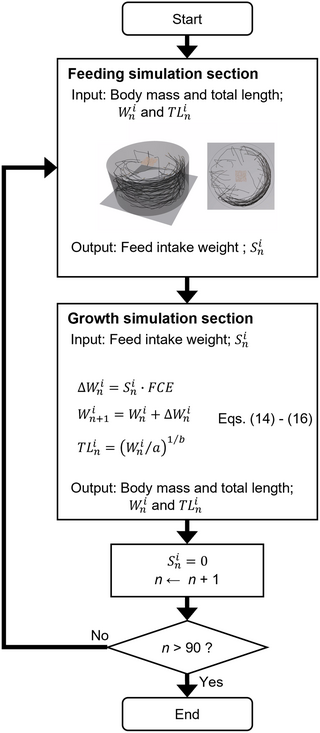
\includegraphics[width=0.3\linewidth]{fig/sim.png}
    \caption{Overview of the simulation model}
    \label{fig:simulation-overview}
\end{figure}

\subsubsection{Growth phase}
After the Feeding Simulation phase, the Growth phase begins, influenced by the fish's food intake. The Feed Conversion Efficiency (FCE), set at 1.0, assumes all ingested food directly contributes to body mass gain, simplifying the relationship between intake and growth.

The fish's body mass update leads to the calculation of the total length using an allometric equation. Additionally, a daily feed intake limit is set at 4\% of the fish's body mass to prevent excessive growth.

The presence of food close to a fish also impacts its movements. When food is present in the tank, it quickly moves towards it. Otherwise, it just swims by following other fish while avoiding boundaries.

Each fish adheres to the following movement model:

\[W_n^i a_{t+\Delta t} = F_t\]
\[v_{t+\Delta t} = v_t +  a_{t+\Delta t}*\Delta t\]
\[x_{t+\Delta t} = x_t + v_{t+\Delta t} *\Delta t\]

Where $W_n$ is the weight of the fish, $a_t$ is its acceleration at instant $t$, $F_t$ is the sum of all the forces driving it at instant $t$, $v_t$ is its speed and $x_t$ its position.

Collectively, fish follow distinct behavioral rules governing separation, alignment, cohesion, approach towards food, boundary avoidance, and random movement. These rules shape dynamic interactions, fostering a nuanced and adaptive system.

To see the details of the equation, refer to the original \cite{article}

\subsection{Setup and visualization of the fish}
We decided to both simulate and visualize the fish behaviour with Godot Engine which is a tool quite similar to Unity. It uses its particular programming language, GDScript, which is Python inspired. For the simulation, we used two classes : Food and Fish. The tank and its details are created in the main so the bulk of the function is in the two first classes.

\begin{itemize}
    \item \textbf{Food} : It sets the weight and the movement of the pellet once dropped into the tank
    \item \textbf{Fish} : This class takes care of simulating the size and behaviour of fish but also the two phases explained above. It manages the modification in behaviour when food is detected by fish, the growth when eating food and the collective behaviour of the school as mentioned.
\end{itemize}   

\section{Results}

Once we completed our implementation, we confirmed that it was correct by running it with the same parameters as in the original paper \cite{article}. Even if we didn't obtained exactly the same values (ours were around 10\% higher), the conclusions we can draw from the data is the same: the size of a square feeding area has no impact on the mean mass of a fish, but it does impact the variance of the sizes. Indeed, with a larger square, the standard deviation is much lower.


The fish's behaviour closely resemble those described in the paper. At the start of the feeding phase, the group forms a school and swims along the tank wall. As soon as the food is in the tank, fish approach, gather, and quickly eat the feed, usually within 5 seconds. After eating, they go back to their usual swimming style, staying close to the tank wall.

We then conducted simulations using shapes that were not present in the original paper (line, cross and circle) but with the same set of sizes (0.5m, 1m and 1.5m). The analysis revealed that regardless of the size and shape of the feeding zone, the mean mass of a fish at the end of the simulation had no significant differences, as shown in Figure \ref{fig:results}. 


However, what did change noticeably was the heterogeneity in fish's weight. Even though the total weight didn't vary much, the differences in how individual fish grew varied more between the feeding areas. This is illustrated in the tables of Figure 4.

This means that while the feeding area didn't hugely affect the total weight gain, it did impact how much the fish growth varied. These variations are much more prevalent when feeding the school using a square area to spread food, using a circle the standard deviation does not change much with the radius of the area.

\begin{figure}[h]
    \centering
    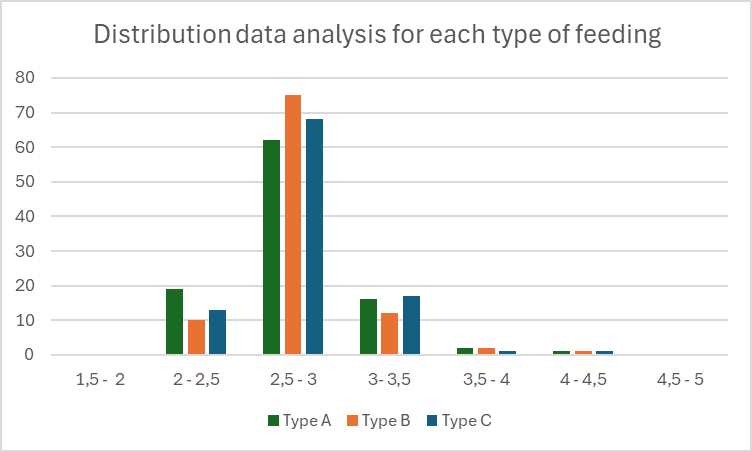
\includegraphics[width=(2in+\columnwidth)/3]{fig/graph_square.png}
    \hfill
    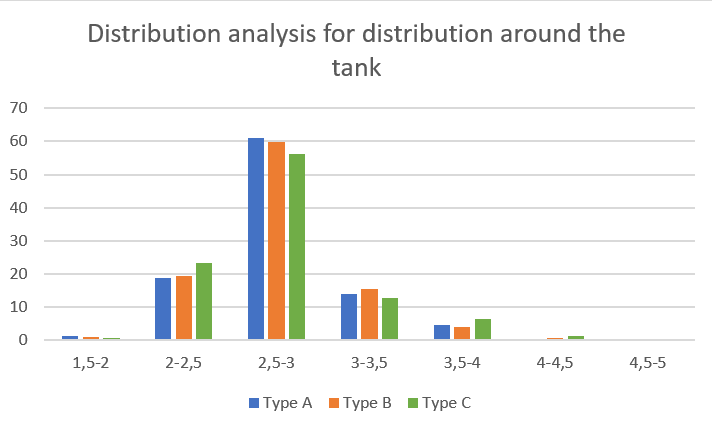
\includegraphics[width=(2in+\columnwidth)/3]{fig/graph_circle.png}
    \caption{Distribution of fish sizes for a square feeding area (as in the original article) and a circular area. Type A, B and C refers to feeding areas of diameter 0.5m, 1m and 1.5m respectively.}
    \label{fig:results}
\end{figure}

\begin{figure}[h]
    \centering
    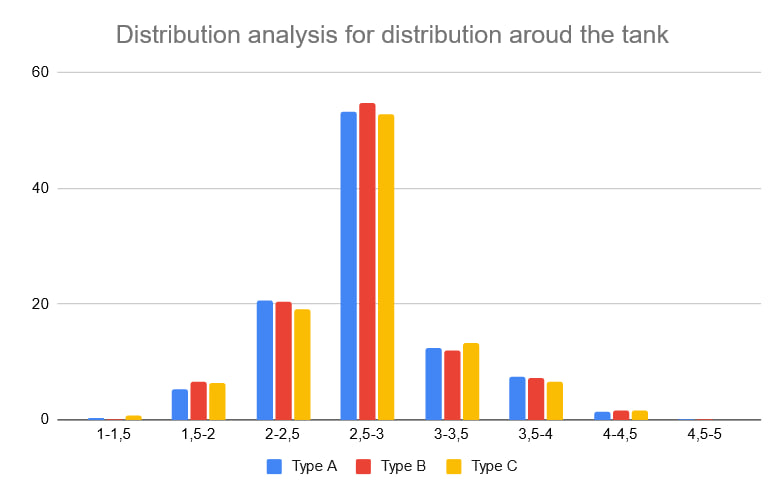
\includegraphics[width=(2in+\columnwidth)/3]{fig/graph_line.jpg}
    \hfill
    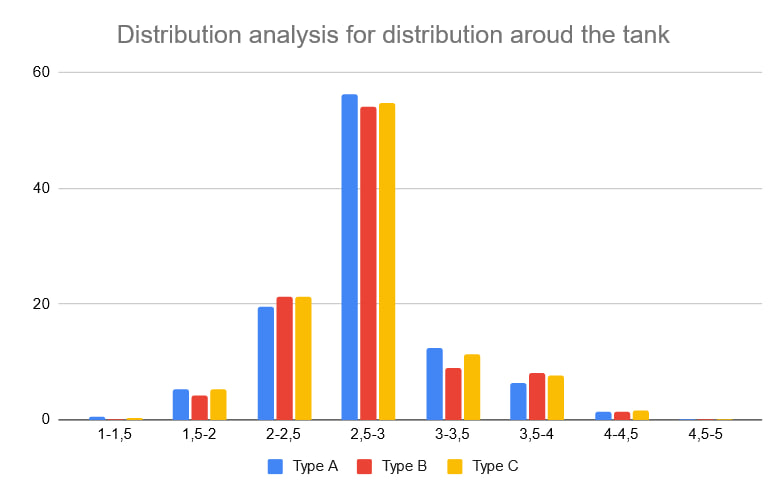
\includegraphics[width=(2in+\columnwidth)/3]{fig/graph_cross.jpg}
    \caption{Distribution of fish sizes for a line shape feeding area and a cross shape area. Type A, B and C refers to feeding areas of diameter 0.5m, 1m and 1.5m respectively.}
    \label{fig:results}
\end{figure}

\begin{figure}[h]
    \centering

    \begin{minipage}{0.45\textwidth}
        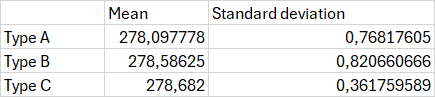
\includegraphics[width=\textwidth]{fig/stats_square.png}
        \caption{Fish sizes for a square feeding area (as in the original article).}
    \end{minipage}
    \hfill
    \begin{minipage}{0.45\textwidth}
        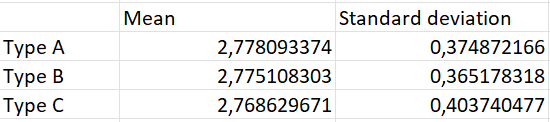
\includegraphics[width=\textwidth]{fig/stats_circle.png}
        \caption{Fish sizes for a circular feeding area.}
    \end{minipage}

    \vspace{\baselineskip} % Vertical space between rows

    \begin{minipage}{0.45\textwidth}
        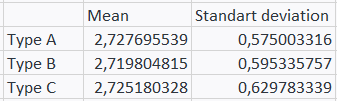
\includegraphics[width=\textwidth]{fig/line.png}
        \caption{Fish sizes for a line-shaped feeding area.}
    \end{minipage}
    \hfill
    \begin{minipage}{0.45\textwidth}
        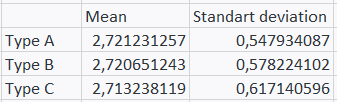
\includegraphics[width=\textwidth]{fig/cross.png}
        \caption{Fish sizes for a cross-shaped feeding area.}
    \end{minipage}

\end{figure}


\section{Discussion}

In a real-world scenario, it would be more logical to start with fish of varied sizes. Given the aquaculture setting, it would also be necessary to permit the removal of mature fish that meet the minimum size requirement for sale. Consequently, smaller fish could then continue to grow.The implementation of this practice would enable a more gradual and continuous production and enhance the realism. 

Nevertheless with the obtained results, we can say  that if we want fish to grow at the same speed, it is better to distribute their food using a circle, a line or a cross rather than a square.


It can be hard to tell why we observe such differences, but one hypothesis is that once a fish starts to eat more than the others, it will continue to be advantaged as we consider that well-fed fish are faster in the simulation. As fish tend to naturally gather in schools that circles around the tank, distributing food in circular fashion better spreads food intake among the fish population. When fed using a square shape at the center of the tank, only fish that are away from the border are able to reach food, and start to take advantage over the other ones.

The \emph{Food Conversion Efficiency} model that is used to determine fish growth depending on the quantity of food they have eaten is also considered to be a poor approximation of how it works in real life. It would be interesting to see which results can be obtained by implementing this part of the simulation differently.

\section{Conclusion }
To summarize what has been done, we have reproduced the model proposed in the original paper. In the simulation we have also implemented different shapes and sizes of the feeding zones, automated food distribution and fish spawning. Our analysis focused on the impact of different feeding areas, leading to the conclusion that a more even distribution of food results in more uniform fish growth. We are aware of the improvements that may be added to our simulation but this extension highlights one of the advantages of using IT and collective behaviour simulation to solve this problem. 

\section{Contributions}
\begin{itemize} 
    \item \textbf{Ana:} Worked on the report, implemented a graphical user interface overlay to control the simulation, reworked the data export, worked on the slides, automated food spawning.

    \item \textbf{Sarah:} Implemented the various feeding shapes. Ran tests and produced graphs for analysis. Worked on the slides and corrected the report.

    \item \textbf{Mélinda:} Also ran tests and produced graphs for analysis. Worked on the slides and corrected the report. Automated fish spawning at the beginning of the simulation. 

    \item \textbf{Alina:} Worked on the report, ran tests and produced graphs.
    
\end{itemize}

    

\begin{multicols}{2}
\section*{\bibname}
% Bibliography
\bibliography{./bib/bibliography}
\end{multicols}

\end{document}